\scanpage{5}

% 1–8, inclusion and incidence
Ceci dit, les relations d'inclusion naturelles entre les $G_n^\delta$ ($G_n^\delta\subset G_n^{\delta'}$ pour $\delta'\subset\delta$) définissent les relations d'incidence \inserted{(= \unsure{prolonger et restreindre|prolongement et restriction|relations d'inclusion})} entre drapeaux de types \deleted{\unsure{$\delta$}} divers. On reconstitue ainsi l'ens ordonné des drapeaux des divers types $\delta$, et par là l'ens des $F_\alpha$ (drapeaux minimaux) et leurs relations d'incidence\ldots.

% 9, transition
De façon précise :

% 10–14, proposition
\uline{Prop} Le foncteur $(F_*)\unsure{\mapsto|\vdash}(\mathcal A)$ des complexes cellulaires satisfaisant les conditions $1,1',2,2',3,4$ (renforcé ?) vers les ens à groupe d'opérateurs $G_n$, est \uline{pl. fidèle}.

% 15–16, essential image
Il faudrait déterminer l'image essentielle.

% after 16, separator
\figure{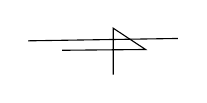
\begin{tikzpicture}[x=1cm,y=1cm]\draw (-.95,0) -- (.95,.03); \draw (-.52,-.12) -- (.54,-.11) -- (.13,.16) -- (.13,-.43);\end{tikzpicture}}

% 17–21, geometric realization
Réalisation géom. d'un complexe $F_{\unsure{\alpha|*}}$ (satisfaisant \unsure{les deux axiomes|le seul axiome} 1) : c'est par définition la réalisation géométrique de la triangulation combinatoire définie par l'ens des parties \inserted{(finies)} tot\textsuperscript{t} ordonnées de \deleted{\unsure{$F$}}$F_*$.

% lower left
% archive sheet number: 4
